\documentclass[tikz]{standalone}
% Timeline library
\usetikzlibrary{backgrounds,calc}
\usepackage{xstring}

\pgfkeys{/tikz/.cd,
  timespan/.store in=\timespan,
  timespan=Week,
  timeline width/.store in=\timelinewidth,
  timeline width=20,
  timeline height/.store in=\timelineheight,
  timeline height=1,
  timeline offset/.store in=\timelineoffset,
  timeline offset=0.15,
  initial week/.store in=\initialweek,
  initial week=1,
  end week/.store in=\endweek,
  end week=2,
  time point/.store in=\timepoint,
  time point=0.5,
  between week/.style args={#1 and #2 in #3}{
    initial week=#1,
    end week=#2,
    time point=#3,
  },
  involvement degree/.store in=\involvdegree,
  involvement degree=2cm,
  phase color/.store in=\phasecol,
  phase color=red!50!orange,
  phase appearance/.style={
    circle,
    opacity=0.3,
    minimum size=\involvdegree,
    fill=\phasecol
  },
}
\pgfkeys{/tikz/milestone/.cd,
  at/.store in=\msstartpoint,
  at=phase-1.north,
  circle radius/.store in=\milestonecircleradius,
  circle radius=0.1cm,
  direction/.store in=\msdirection,
  direction=90:2cm,
  text/.store in=\mstext,
  text={},
  text options/.code={\tikzset{#1}},
}

\newcommand{\reftimespan}{\MakeLowerCase{\timespan}}

\newcommand{\timeline}[1]{
  \draw[fill,opacity=0.8] (0,0) rectangle (\timelinewidth,\timelineheight);
  \shade[top color=black, bottom color=white,middle color=black!20]
    (0,0) rectangle (\timelinewidth,-\timelineoffset);
  \shade[top color=white, bottom color=black,middle color=black!20]
    (0,\timelineheight) rectangle (\timelinewidth,\timelineheight+\timelineoffset);

  \foreach \smitem [count=\xi] in {1,...,#1} {\global\let\maxsmitem\xi}
  \pgfmathsetmacro\position{\timelinewidth/(\maxsmitem+1)}
  \node at (0,0.5\timelineheight)(\timespan-0){\phantom{Week 0}};

  \foreach \x[count=\xi] in {1,...,#1}{
      \node[text=white]at +(\xi*\position,0.5\timelineheight) (\timespan-\xi) {\timespan\ \x};
  }
}

\newcounter{involv}
\setcounter{involv}{0}

\newcommand{\phase}[1]{
\stepcounter{involv}
\node[phase appearance,#1]
(phase-\theinvolv)
at ($(\timespan-\initialweek)!\timepoint!(\timespan-\endweek)$){};
}

\newcommand{\initialphase}[1]{
\node[phase appearance,#1,anchor=west,between week=0 and 1 in 0,]
(phase-\theinvolv)
at ($(\timespan-0)!0!(\timespan-1)$){};
\setcounter{involv}{0}
}

\newenvironment{phases}{\begin{pgfonlayer}{background}}{\end{pgfonlayer}}

\newcommand{\addmilestone}[1]{
\pgfkeys{/tikz/milestone/.cd,#1}
\draw[double,fill] (\msstartpoint) circle [radius=\milestonecircleradius];
\draw(\msstartpoint)--++(\msdirection)node[/tikz/milestone/text options]{\mstext};
}
%%%%%%%%%%%%%%%%%%%%%%%%%%%%%%%%%%%%%%%%%%%%%%%%%%%%%%%%%%%%%%%%%%%%%%%%%%%%%%%


% redefinition for having a interval not starting from 1
\renewcommand{\timeline}[1]{
  \draw[fill,opacity=0.8] (0,0) rectangle (\timelinewidth,\timelineheight);
  \shade[top color=black, bottom color=white,middle color=black!20]
    (0,0) rectangle (\timelinewidth,-\timelineoffset);
  \shade[top color=white, bottom color=black,middle color=black!20]
    (0,\timelineheight) rectangle (\timelinewidth,\timelineheight+\timelineoffset);

  \foreach \smitem [count=\xi] in {#1}  {\global\let\maxsmitem\xi}
  \pgfmathsetmacro\position{\timelinewidth/(\maxsmitem+1)}
  \node at (0,0.5\timelineheight)(\timespan-0){\phantom{Week 0}};

  \foreach \x[count=\xi] in {#1}{
      \node[text=white]at +(\xi*\position,0.5\timelineheight) (\timespan-\xi) {\timespan\ \x};
  }
}

\begin{document}

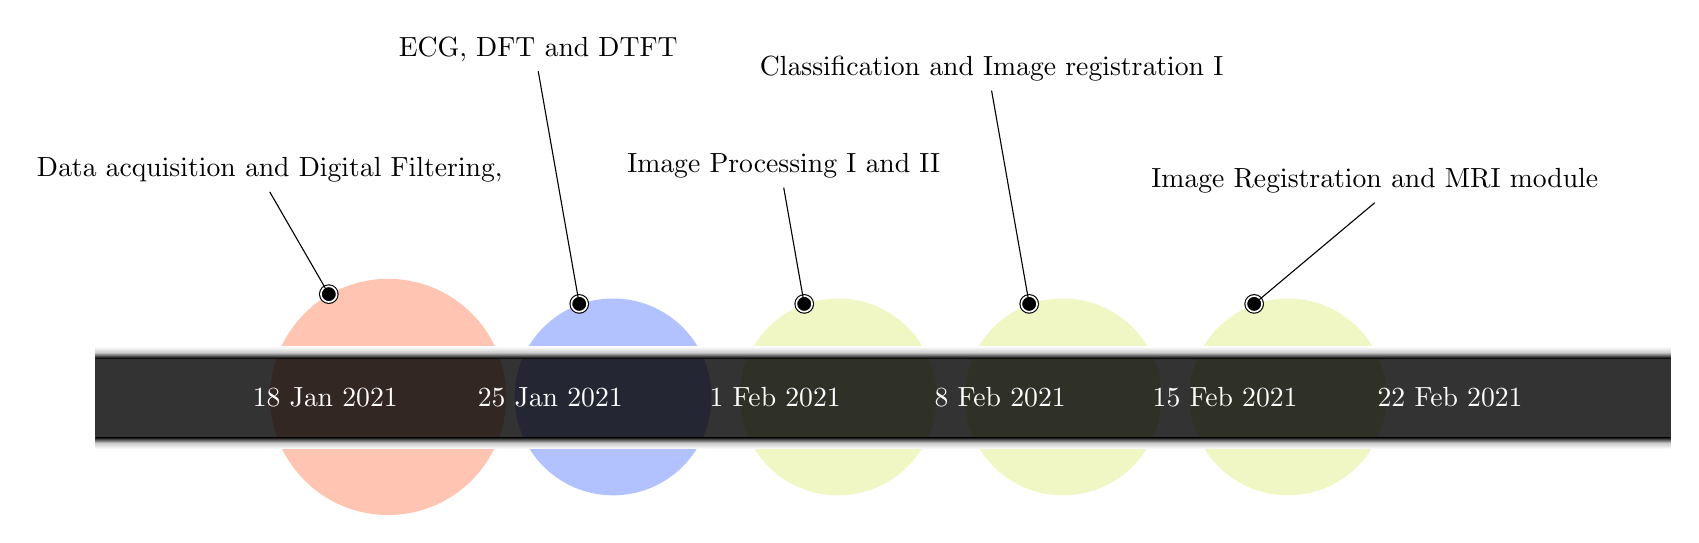
\begin{tikzpicture}[timespan={},% empty to not display a label before the month
  between month/.style args={#1 and #2 in #3}{% auxiliary style for month
    initial week=#1,
    end week=#2,
    time point=#3,
  }
  ]
\timeline{18 Jan 2021, 25 Jan 2021,1 Feb 2021, 8 Feb 2021, 15 Feb 2021, 22 Feb 2021} % months

% put here the phases
\begin{phases}
\phase{between month=1 and 2 in 0.3,involvement degree=3cm}
\phase{between month=2 and 3 in 0.3,phase color=blue!80!cyan, involvement degree=2.5cm}

\phase{between month=3 and 4 in 0.3,phase color=yellow!80!cyan, involvement degree=2.5cm}

\phase{between month=4 and 5 in 0.3,phase color=yellow!80!cyan, involvement degree=2.5cm}

\phase{between month=5 and 6 in 0.3,phase color=yellow!80!cyan, involvement degree=2.5cm}

\end{phases}

% put here the milestones
\addmilestone{at=phase-1.120,direction=120:1.5cm,text={Data acquisition and Digital Filtering,},text options={above}}

\addmilestone{at=phase-2.110,direction=100:3cm,text={ECG, DFT and DTFT},text options={above}}

\addmilestone{at=phase-3.110,direction=100:1.5cm,text={Image Processing I and II},text 
options={above}}

\addmilestone{at=phase-4.110,direction=100:2.75cm,text={Classification and Image registration I},text 
options={above}}

\addmilestone{at=phase-5.110,direction=400:2cm,text={Image Registration and MRI module},text 
options={above}}


\end{tikzpicture}
\end{document}